\chapter{Network I/O Contention}\label{chapter:network}

\section{Throughput}


\section{Methodology}

\subsection{Latency}
For latency benchmarking, we employed both \textit{iPerf3} and \textit{sockperf} \cite{sockperf}. 
Sockperf is a network benchmarking utility capable of measuring the latency of packets with a 
sub-nanosecond resolution. It introduces minimal overhead by leveraging the Time Stamp Counter (TSC) 
registers that count the number of CPU cycles for measuring latency \cite{sockperf}. \\
Sockperf requires a client-server setup as well: the client sends mutliple packets to the server
, receives responses and records the \ac{RTT} for each packet. 
The tool provides different options to visualize the results with varying granularity. 
A CSV file is generated listing the send and response times for each individual packet,
along with a report of the average latency and key metrics such as the 90th and 99th percentile. \\
The objective of the latency experiment was to evaluate the effect of increasing aggregate throughput 
utilization of neighbors on the latency of the test node. The experiment
consists of the following steps: Similar to the throughput experiment, we deploy two dedicated hosts, 
one hosting all clients and one hosting all servers. Initially, only the client test node 
and its corresponding server are created. We measure the latency between them and record it as a baseline 
value. After that, we deploy all the remaining clients and incrementally increase their aggregate 
throughput usage in 1 Gbit/s steps (or smaller as we notice the presence of latency degrdation).
This is possible through an iPerf3 functionality that allows the specification of an exact throughput 
value for the client, allowing us to control the aggregated throughput of the neighbors.
The test client node and its corresponding server are the only nodes using the sockperf tool. 
Since all dedicated hosts, including the client test node and server, are located within 
the same \ac{AZ} (See Chapter \ref{chapter:infra}), 
external latency variability is minimized, allowing for a better identification of latency degradation. \\
The overall architecture of the latency experiment is similar to Figure \ref{fig:netexp}. The two 
key differences are: (i) the test pair (client and server) used sockperf instead of iPerf3, and 
(ii) The neighboring nodes did not immediately saturate the available bandwidth, 
but instead progessively increased their throughput. 


\section{Throughput Contention}
\subsection{m5 family}
Unlike other resources such as CPU and RAM, which are statically divided between the different tenants 
based on instance type, network bandwidth is shared among the different co-tenants without a fix
specification of the expected bandwidth per tenant. Typically, for instances with 16 vCPUs or less, 
AWS specifies the bandwidth upper bound, e.g., "Up to 10 Gbps" \cite{network_bandwidth}. However these 
instances still have a baseline bandwidth. A network I/O credit mechanism is then employed that 
allows the instance to use burst bandwidth for a short period of time, ranging from 5 to 60 minutes,
depending on the instance type \cite{network_bandwidth}. \\ 
In this section, we'll analyze throughput contention on instances belonging to the m5 family. Key
performance metrics for the m5 dedicated host can be found in Table \ref{tab:dedicated-hosts}.
Table \ref{tab:m5_spec} depicts the most important network related specifications for the different 
instance types.
\begin{table}[H]
\centering
\begin{tabular}{lccc}
\toprule
\textbf{Type} & \textbf{vCPUs} & \textbf{Burst BW (Gbps) \cite{cloudspecs}} & \textbf{Baseline BW \cite{cloudspecs}} \\
\midrule
m5.large     & 2  & 10 & 0.75 \\
m5.xlarge    & 4  & 10 & 1.25 \\
m5.2xlarge   & 8  & 10 & 2.5  \\
m5.4xlarge   & 16 & 10 & 5    \\
m5.8xlarge   & 36 & 10 & 10   \\
m5.12xlarge  & 72 & 12 & 12   \\
m5.metal     & 96 & 25 & 25   \\
\bottomrule
\end{tabular}
\caption{Specifications of m5 Instance Types (BW = Bandwidth)}
\label{tab:m5_spec}
\end{table}
\noindent
For single flow traffic, the maximum burst bandwidth of 10 Gbps is only attainable when the the client and 
the server reside in the same cluster group. For instances who are not in the same cluster group, single flow 
traffic is limited to 5 Gbps \cite{network_bandwidth}.  The clients and the servers 
can't be in the same cluster groups since they are in different dedicated hosts. This means that the 
single-flow traffic between the client and the servers is limited to 5 Gbps. To bypass this restriction, 
we create two client connections, that can be achieved using the P option in the iPerf3 tool. \\
Bandwidth throttling for smaller instances takes at least 5 minutes to take effect, during which the instance
has access to 10 Gbps burst bandwidth. We conduct our experiments in this time window. It is particularly 
interesting to observe the extent of the network degradation in comparison to the baseline bandwidth 
for each instance size. The first experiment features the m5.4xlarge instance type, 
of which the dedicated host can accomoadate 6. To provide a better 
visualization of the results, we present each node in an independent graph.
\begin{figure}[H]
\centering
\begin{tikzpicture}
\begin{groupplot}[
    group style={
        group size= 2 by 4,
        horizontal sep=1.25cm,
        vertical sep=1.25cm,
        xlabels at= edge bottom,
        ylabels at=edge left,
    },
    width=6cm,
    height=4cm,
    xlabel={Number of Nodes},
    ylabel={Throughput},
    title style={yshift=-1ex},
    ymin=2, ymax=10,
    xtick distance = 1, 
    xmin=0,
    grid=both,
]

% Node 1
\nextgroupplot[title={Node 1}]
\addplot[mark=*, blue, thick] coordinates {(0,9.96)(1,9.96) (2,8.06)(3,5.97) (4,4.90) (5, 4.01)};

% Node 2
\nextgroupplot[title={Node 2},]
\addplot[mark=square*, red, thick] coordinates {(1,9.96) (2,7.83)(3,5.97) (4,4.98) (5, 4.17)};
% Node 3
\nextgroupplot[title={Node 3}]
\addplot[mark=triangle*, green, thick] coordinates {(2,8.00) (3,5.98) (4,4.91) (5, 4.17)};


\nextgroupplot[title={Node 4}]
\addplot[mark=diamond*, orange, thick] coordinates {(3,5.96) (4, 4.98) (5,3.99)};

% Node 4
\nextgroupplot[title={Node 5}, xlabel={Number of Nodes}]
\addplot[mark=diamond*, orange, thick] coordinates {(4,4.91) (5, 4.11)};

% Node 4
\nextgroupplot[title={Node 6}, xlabel={Number of Nodes}]
\addplot[mark=diamond*, orange, thick] coordinates {(5,4.25)};
\end{groupplot}
\end{tikzpicture}
\caption{UDP Throughput of m5.4xlarge nodes when incrementally increasing the tenants}
\end{figure}

\noindent
As expected, the first and the second clients, when alone on the dedicated host had access to a burst 
bandwidth of 9.96 Gbps. The third tenant caused the average throughput to drop to 7.96 Gbps, while the 
addition of a fourth neighbor further reduced it to 5.96 Gbps. We practically notice no variation between 
the different nodes. The fifth neighbor reduced the throughput of all the co-tenants to practically 
the baseline width of the m5.4xlarge (5 Gbps) with an average throughput of 4.94 Gbps. The 6th node 
introduced the first significant decrease under the baseline width to an average of 4.12 Gbps, 
which is 17.6\% less than the baseline width. Starting from the the 3rd tenant, the sum 
of the throughput across all the nodes is always around 24.7 Gbps.  This was expected as the bandwidth 
of the m5.metal is 25 Gbps, which should represent the upper limit for the sum of the throughputs of all the nodes
residing on the same dedicated host. For the xlarge, 2xlarge, and 4xlarge types, the product of the 
maximum number of the instances on the dedicated host multiplied by the baseline width of the respective
instance type (5 Gbps) is 30 Gbps, which is 16.7\% smaller than the possible bandwidth of 25 Gbps. 
This explains the average degradation of 17\% we saw in the previous experiment. The same behavior
should be expected when using xlarge and 2xlarge instances. For the large instance type, however, the 
product is equal to
\begin{math} 48 \times 0.75 = 36\end{math} Gbps. 
25 Gbps is 30\% smaller than 36 Gbps. We should expect to see an average 
degradation of around 30\% at full capacity if we repeat the experiment using m5.large instances. 
We verify this assumption in the next experiment. Since the dedicated host can host 48 of m5.large 
instances, we can't individually plot the graph of each instance. We used a plotbox graph to display the 
distribution of the throughputs at the different levels. We also used a step size of 8 neighbors, to be 
able to present the results in one graph. 

\begin{figure}[H]
\centering
\begin{tikzpicture}
\begin{axis}[
    boxplot/draw direction=y,
    ylabel={Throughput},
    xlabel={Number of Nodes},
    xtick={1,2,3,4,5,6, 7, 8},
    xticklabels={8, 16, 24, 32, 40, 48},
    ymin = 0.2,
    ymax = 4,
    width=11cm,
    height=7cm,
    grid = both,
]


%\addplot+[
%    boxplot,
%    draw=black,
%] table[row sep=\\, y index=0] {
%data \\
%9.96 \\ 
%}; 

% Boxplot A
\addplot+[
    boxplot,
    draw=black,
] table[row sep=\\, y index=0] {
data \\
2.19 \\ 2.17 \\ 2.19 \\ 3.19 \\ 3.88 \\ 3.17 \\ 3.87 \\ 3.21 \\
};

% Boxplot B
\addplot+[
    boxplot,
    draw=black,
] table[row sep=\\, y index=0] {
data \\
1.12 \\ 1.12 \\ 1.12 \\ 1.82 \\ 2.03 \\ 1.82 \\ 2.00 \\ 1.80 \\ 
1.12 \\ 1.12 \\ 1.18 \\ 2.13 \\ 1.18 \\ 1.19 \\ 1.12 \\ 1.97 \\
};

% Boxplot C
\addplot+[
    boxplot,
    draw=black,
] table[row sep=\\, y index=0] {
data \\
0.86 \\ 0.86 \\ 0.86 \\ 1.16 \\ 1.21 \\ 1.16 \\ 1.20 \\ 1.14 \\ 
0.86 \\ 0.86 \\ 0.86 \\ 1.25 \\ 0.86 \\ 0.85 \\ 0.86 \\ 1.18 \\ 
0.85 \\ 0.85 \\ 1.14 \\ 0.86 \\ 1.13 \\ 0.86 \\ 0.86 \\ 1.27 \\
};

% Boxplot D
\addplot+[
    boxplot,
    draw=black,
] table[row sep=\\, y index=0] {
data \\
0.75 \\ 0.75 \\ 0.75 \\ 0.75 \\ 0.75 \\ 0.75 \\ 0.75 \\ 0.75 \\ 
0.75 \\ 0.75 \\ 0.75 \\ 0.75 \\ 0.75 \\ 0.75 \\ 0.75 \\ 0.75 \\ 
0.75 \\ 0.75 \\ 0.75 \\ 0.75 \\ 0.75 \\ 0.75 \\ 0.75 \\ 0.75 \\ 
0.75 \\ 0.75 \\ 0.75 \\ 0.75 \\ 0.75 \\ 0.75 \\ 0.75 \\ 0.75 \\
};
% Boxplot E
\addplot+[
    boxplot,
    draw=black,
] table[row sep=\\, y index=0] {
data \\
0.28 \\ 0.28 \\ 0.27 \\ 1.15 \\ 0.84 \\ 0.85 \\ 0.84 \\ 1.10 \\ 
0.31 \\ 0.29 \\ 0.21 \\ 1.14 \\ 0.21 \\ 0.19 \\ 0.31 \\ 0.87 \\ 
1.11 \\ 1.09 \\ 1.22 \\ 1.26 \\ 1.20 \\ 0.29 \\ 1.59 \\ 1.46 \\ 
0.23 \\ 0.20 \\ 0.55 \\ 0.53 \\ 0.44 \\ 0.54 \\ 0.26 \\ 0.52 \\ 
0.26 \\ 0.23 \\ 0.82 \\ 0.78 \\ 0.21 \\ 0.20 \\ 0.22 \\ 0.21 \\
};
% Boxplot F
\addplot+[
    boxplot,
    draw=black,
    solid,
] table[row sep=\\, y index=0] {
data \\
0.70 \\ 0.67 \\ 0.14 \\ 0.98 \\ 0.76 \\ 0.74 \\ 0.59 \\ 0.94 \\ 
0.13 \\ 0.71 \\ 0.28 \\ 0.58 \\ 0.18 \\ 0.17 \\ 0.13 \\ 0.60 \\ 
0.16 \\ 0.19 \\ 0.96 \\ 0.20 \\ 0.97 \\ 0.15 \\ 0.70 \\ 0.89 \\ 
0.19 \\ 0.18 \\ 0.76 \\ 0.89 \\ 0.97 \\ 0.88 \\ 0.72 \\ 0.76 \\ 
0.14 \\ 0.75 \\ 0.62 \\ 0.20 \\ 0.20 \\ 0.18 \\ 0.23 \\ 0.18 \\ 
0.16 \\ 0.57 \\ 0.58 \\ 0.92 \\ 0.75 \\ 0.56 \\ 0.15 \\ 0.58 \\
};
\end{axis}
\end{tikzpicture}
\caption{Throughput (UDP) of m5.large nodes when incrementally increasing the number tenants}
\end{figure}
\noindent
The first node has access to a throughput of 9.96 Gbps, which represents the maximum burst bandwidth. 
At 8 neighbors, the average throughput drops to 3 Gbps. We then observe a gradual degradation 
with an average of 1.5 Gbps at 16 nodes, 1 Gbps at 24 nodes, and  0.75 Gbps at 32 nodes,  which corresponds 
to the baseline bandwidth of the m5.large instance type. 
At this level, we interestingly notice zero variation between the 
different co-tenants. At 40 nodes, the average decreases to 0.614 Gbps and further to 0.51 Gbps at 48 nodes.  
At full capacity, The average throughput (0.51 Gbps) is 30.7\% lower than the baseline bandwidth of the 
m5.large instance (0.75 Gbps). This more significant performance degradation close to 30\% was expected 
as hypothesized earlier. In this experiment, we also observe an important performance variation 
between the different nodes compared to the previous experiment.

\section{Latency}
\subsection{m5 family}
\begin{figure}[ht]
\centering
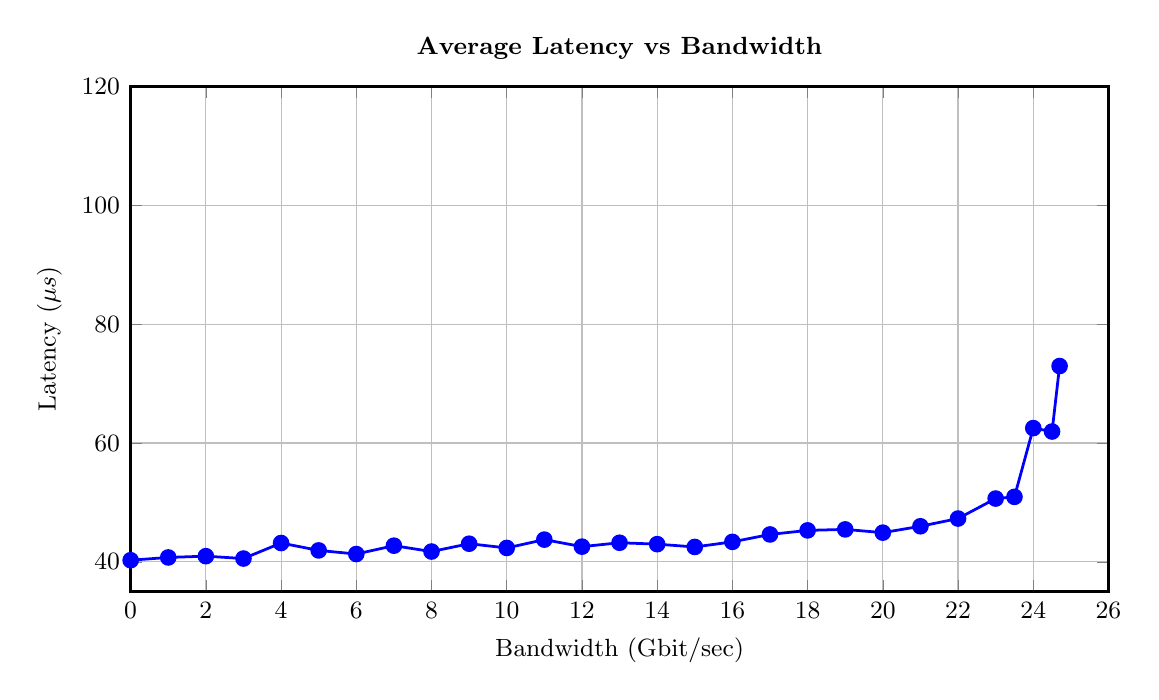
\begin{tikzpicture}
\begin{axis}[
    width=14cm,
    height=8cm,
    xlabel={Bandwidth (Gbit/sec)},
    ylabel={Latency (\(\mu s\))},
    title={Average Latency vs Bandwidth},
    grid=major,
    xmin=0, xmax=26,
    ymin=35, ymax=120,
    xtick={0,2,...,25.5},
    ytick={40,60,...,120},
    line width=1pt,
    mark size=2.5pt,
    tick label style={font=\small},
    label style={font=\small},
    title style={font=\bfseries\small},
]
\addplot[
    color=blue,
    mark=*,
]
coordinates {
    (0, 40.281)
    (1, 40.750)
    (2, 40.962)
    (3, 40.562)
    (4, 43.174)
    (5, 41.930)
    (6, 41.321)
    (7, 42.730)
    (8, 41.737)
    (9, 43.058)
    (10, 42.344)
    (11, 43.749)
    (12, 42.563)
    (13, 43.221)
    (14, 42.983)
    (15, 42.511)
    (16, 43.369)
    (17, 44.616)
    (18, 45.298)
    (19, 45.465)
    (20, 44.918)
    (21, 45.990)
    (22, 47.289)
    (23, 50.653)
    (23.5, 50.938)
    (24, 62.502)
    (24.5, 61.927)
    (24.7, 72.939)
};
\end{axis}
\end{tikzpicture}
\caption{Average Latency vs Bandwidth}
\end{figure}

\subsection{c7g family}
\section{Discussion}